\documentclass[en]{../../../eplsummary}
\usepackage{framed}
\usepackage{placeins}
\usepackage{listings}
\usepackage{color}

\definecolor{dkgreen}{rgb}{0,0.6,0}
\definecolor{gray}{rgb}{0.5,0.5,0.5}
\definecolor{mauve}{rgb}{0.58,0,0.82}

\lstset{frame=tb,
  language=Java,
  aboveskip=3mm,
  belowskip=3mm,
  showstringspaces=false,
  columns=flexible,
  basicstyle={\small\ttfamily},
  numbers=none,
  numberstyle=\tiny\color{gray},
  keywordstyle=\color{blue},
  commentstyle=\color{dkgreen},
  stringstyle=\color{mauve},
  breaklines=true,
  breakatwhitespace=true,
  tabsize=3
}

\graphicspath{{res/}}

\hypertitle{algo-INGI2266}{7}{INGI}{2266}
{Houtain Nicolas}
{de Vogelaere Cyril}
{Pierre Schaus}

\section{Dynamic programing}

\subsection{Definition}

\textbf{Dynamic programming} is a method by recurrence in order to solve complex problem.
\begin{itemize}
    \item breaking it down into a collection of simpler subproblems
    \item solving each of those subproblems just once, and storing their solutions in memory
    \item[$\rightarrow$] Next time the same subproblem occurs, instead of 
recomputing its solution, only looks up to the previously computed solution.
Thereby \textbf{saving computation time at the expense of storage space}.
\end{itemize}

\subsection{Solving the knapsack problem with DP}

\subsubsection{The knapsack problem}
\begin{itemize}
    \item A set of item $I$
    \item for each item $i \in I$ is associated a value $v_i$ and a weight $w_i$.

    \item[Goals] 
        \begin{tabular}{m{3cm}m{12cm}}
            $\sum_{i \in I} v_i x_i$: & Maximize the value of selected items\\
            $\sum_{i \in I} w_i x_i \le C$ & Under constraint that the total
            capacity cannot exceed a given maximal capacity $C$ \\ 
            $x_i \in \{0,1\}$ & And an item cannot be partially selected \\
        \end{tabular}
\end{itemize}

Note that Knapsack is an NP-Complete problem as it can be used
to find a solution to the subset-sum problem, which is NP-complete.

\paragraph{Subset-sum problem}

Given a set of natural number and a capacity K. 
Find a subset S such that :
$$\sum_{i \in S} c_i = K$$


\subsubsection{Solutions}
\begin{itemize}
    \item \textbf{DP for knapsack in 0(Cn)}.

        Refer to the optimal objective of the problem with capacity $k$ and
        items \{1,…,j\} $\in$ I as $O(k,j)$. We can easily notice that :

        \begin{itemize}
            \item $O(k,0) = 0 \text{\footnotemark}$
            \item $ O(k,j) = \begin{cases} 
                    max(O(k,j-1) , vj +O(k-wj,j-1))\text{\footnotemark} & if \quad w_j \leq k \\
                    O(k,j-1) & otherwise
                \end{cases}$
        \end{itemize}
        \footnotetext{As their are no elements to choose from}
        \footnotetext{Bellman's equations}


        \begin{lstlisting}[caption=Knapsack DP]
val items = Array((1,1),(6,2),(18,5),(22,6),(28,7)) // (value,weight)
val C = 11
def O(j: Int, k: Int): Int = {
    if (j < 0) 0
    else {
        val (vj,wj) = items(j)
        if (wj > k) O(j-1,k)
        else O(j-1,k).max(vj + O(j-1,k-wj))
    }
}
println(O(items.size-1,C))
        \end{lstlisting}

        \begin{center}
    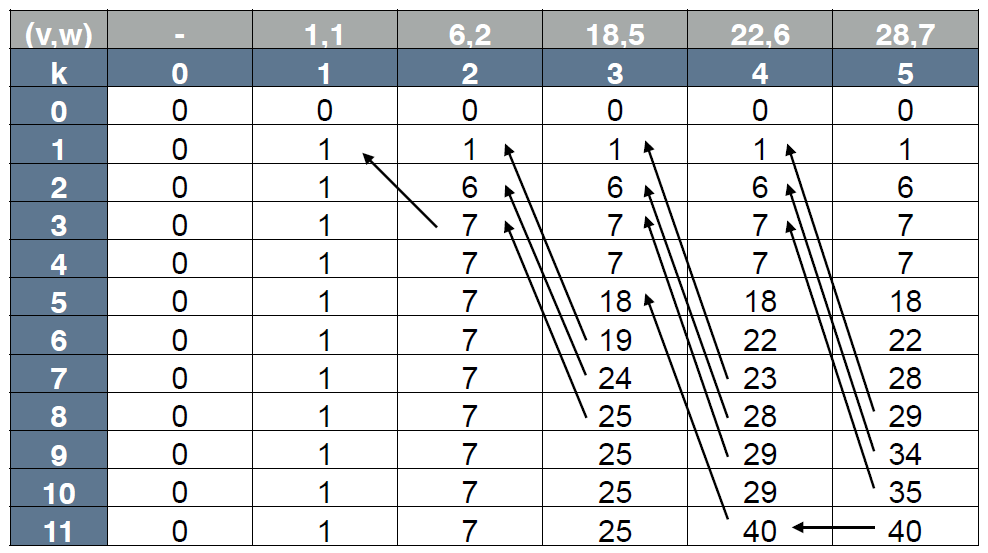
\includegraphics[width=7cm]{KnapsackDP.png}
        \end{center}

    \item \textbf{DP for knapsack in 0(Vn)}.

        Using a similar logic, it is also possible to define an algorithm which
        run in $\theta$(Vn) to compute knapsacks. Let $V = \sum_{i \in I} v_i$,
        we can redefine O(k,j) as O(w,j), the optimal weight using only items
        \{1,...,j\}. The equation will thus change as follow :

    \begin{itemize}
    \item $O(0,j) = O(p,0) = 0 \text{\footnotemark} $
    \item $ O(p,j) = \begin{cases}
                min(O(p,j-1), wi + O(p-v_j,j-1)) & if \quad v_j \leq p \\
                O(p,j-1) & otherwise
            \end{cases}$
        \end{itemize}
        \footnotetext{As $w_i > 0$ for all $i \in I$ and as we cannot have w > 0 with 
        an empty set.}
        \begin{center}
            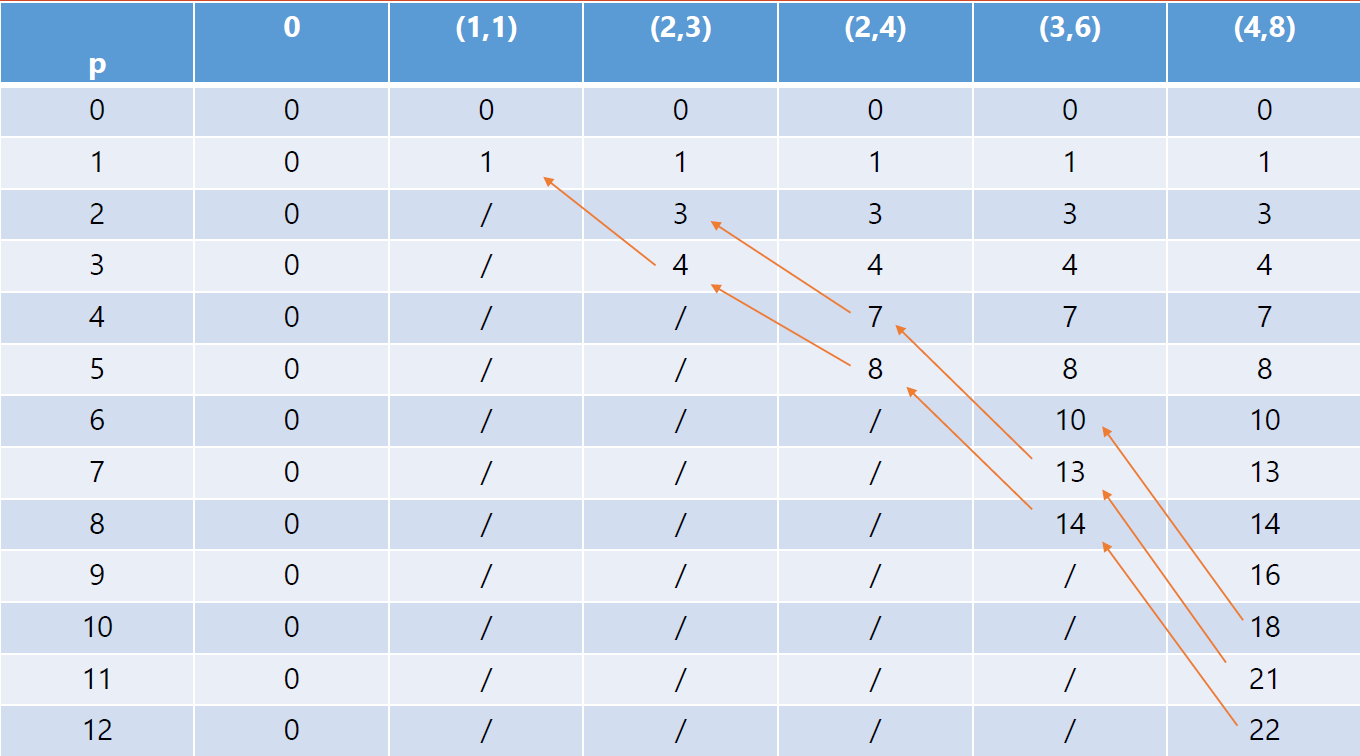
\includegraphics[width=7cm]{KnapsackDPAlgo2.png}
        \end{center}
\end{itemize}

\subsubsection{Cache usage}
\begin{tabular}{m{9cm}m{6cm}}
As explain, a cache is use in order to store computed value and avoid to recompute
it. In \textcolor{red}{red} we have the cells actually computed.
&
    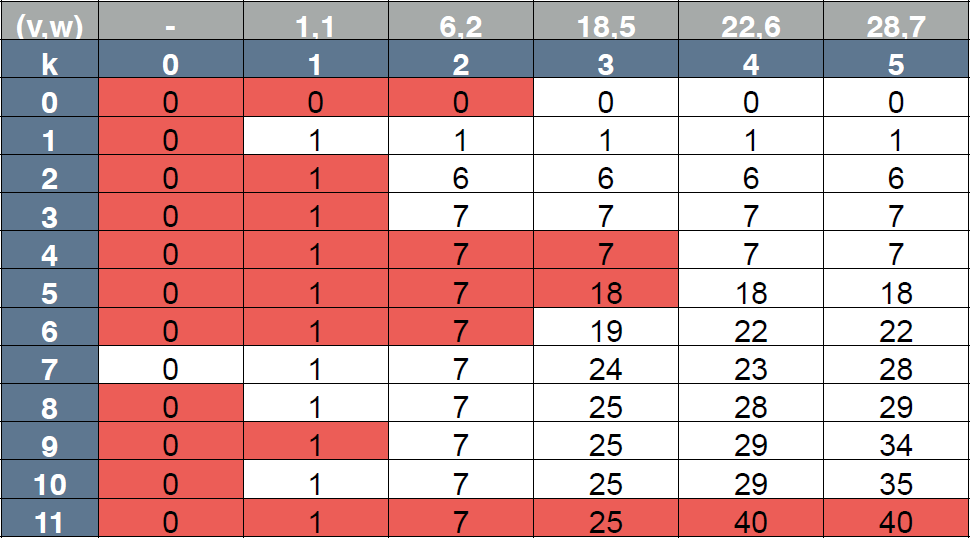
\includegraphics[width=6cm]{KnapsackDPAlgo1.png}
\end{tabular}


\subsubsection{Pseudo-polynomial}

DP is \textsc{pseudo-polynomial}, since it is exponential in the 
\textit{length of input} ($log(C)$) which is the number of bits required to
encode the input ($C$). The complexity is thus exponential relatively to the
input size. This algorithm is \textbf{weakly NP-Complete} or
\textbf{pseudo-polynomial}\footnote{a numeric algorithm runs in
pseudo-polynomial time if its running time is polynomial in the numeric value
of the input, but is exponential in the length of the input – the number of
bits required to represent it.} as it is roughly polynomial for small values of
C while computing larger value is much more expensive\footnote{Not all
    NP-Complete algorithm are pseudo polynomial ! Like the traveling salesman
problem (TSP), for example.}.


\subsection{Other examples of DP algorithms}

Before reading this section, please remember that all algorithm that can be
implemented via dynamic programming are not ipso-facto pseudo polynomial ! Any
algorithm can be expressed with dynamic programming as long as it can be separated in
sub problems.

%\subsubsection{TSP}
%Say $1$ be the source of the TSP.
%\begin{itemize}
%    \item $O(S,1) = 0 $
%    \item $ O(S, j) = 
%        min\Bigg( \{ \quad O\bigg(S -\{j\}, i\bigg) + d_{ij} \quad
%            |\quad  i \in S \wedge i \in
%        Neighboor(j)\quad \} \Bigg)$
%\end{itemize}
%
%The answer to join $1$ to $n$ is $O(AllVertex, n)$


\subsection{Exam}
I give you a problem (for instance the TSP, Knapsack)
\begin{itemize}
    \item  Design a greedy algorithm
    \item  Design a Dynamic Programming formulation
    \item  Design a relaxation and upper/lower bound
        procedure and embed it in a Branch and Bound
    \item  Justify advantages and disadvantages of each
    \item  Apply the three techniques to a small instance
        manually
\end{itemize}



\section{Branch and bound}

\subsection{Definition}

A \textbf{branch-and-bound} algorithm consists of a systematic enumeration of
candidate solutions by means of state space search: the set of candidate
solutions is thought of as forming a rooted tree with the full set at the root.

\begin{itemize}
    \item Explores branches of this tree, which represent subsets of the
solution set. 
    \item Note that before enumerating the candidate solutions of a branch, the
branch is checked against upper and lower estimated bounds on the optimal
solution, and is discarded if it cannot produce a better solution than the best
one found so far by the algorithm.
\end{itemize}

\subsection{Solving the knapsack problem with B\&B}

Given the following knapsack problem :
    \begin{tabular}{cl}
        maximize & $28x_1+30x_2 +20x_3$\\
        subject to & $4x_1+6x_2 +4x_3 \leq 9$\\
                   & $x_i \in \{0, 1\} \forall i$
    \end{tabular}

\subsubsection{Relaxation}
We can choose to relax in order to reduce the search space as much as possible.

\begin{enumerate}
    \item \textbf{Capacity relaxation}: Relax on the constraint by don't
        explore branch which already violated the constraint.

        $\Rightarrow$ Cut at tree branch when 
        we have surpassed the capacity.
        \begin{center}
        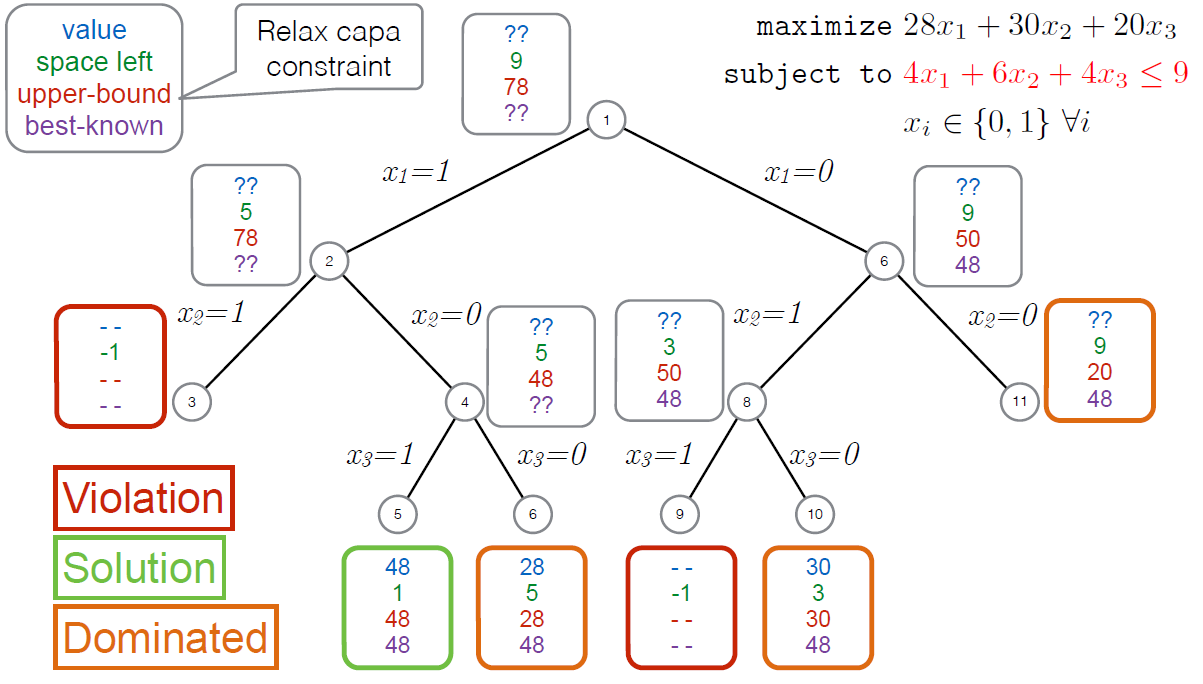
\includegraphics[width=12cm]{KnapsackBBCapaRelaxation.png}
        \end{center}
        It is far from optimal as our upper bound are not close enough to their real
        value.

    \item \textbf{Linear relaxation}: Relax on the value to maximize by
        calculating an upper bound and don't explore if the upper bound <
        actual best value.

        \paragraph{Upper bound computation}
        Given a set sorted by ratio $v_i/w_i$,
        \begin{eqnarray*}
            j &= min\{i \in I: \sum_{k \in 1,...,i} w_k > C\}\\
            UB &= \sum_{i<j} v_i + \frac{(C - \sum_{i \in 1..j-1} w_i)}{w_j} v_j
        \end{eqnarray*}

        $j$ is called the critical item which is in fact the first item (sorted by better ratio)
        which cannot be add entirely, so we just add the ratio of the item according to 
        the free space.

        \begin{center}
            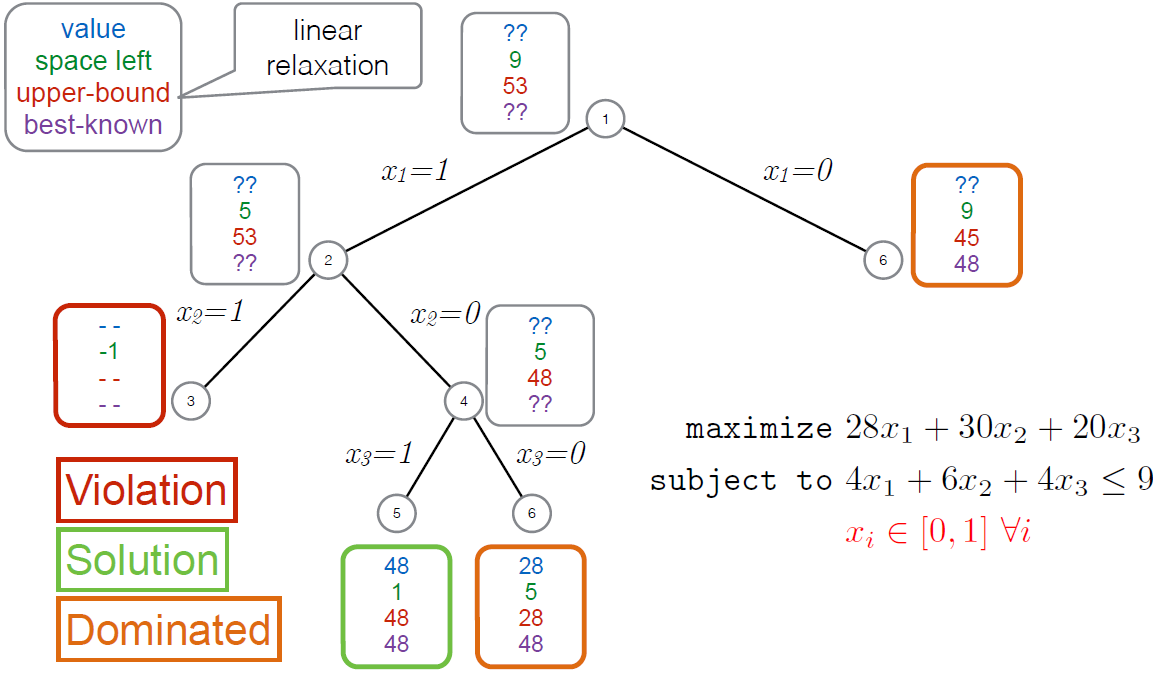
\includegraphics[width=12cm]{KnapsackBBLinearRelaxation.png}
        \end{center}

        Improving the precision of the upper-bound yields far better
        result. Take care however not to over/under estimate it (depending if you are
        on a maximisation or minimisation process) as it might prevent you to find the
        optimal solution.

\end{enumerate}


\subsection{B\&B pseudo-code}

\begin{figure}[!ht]
    \centering
    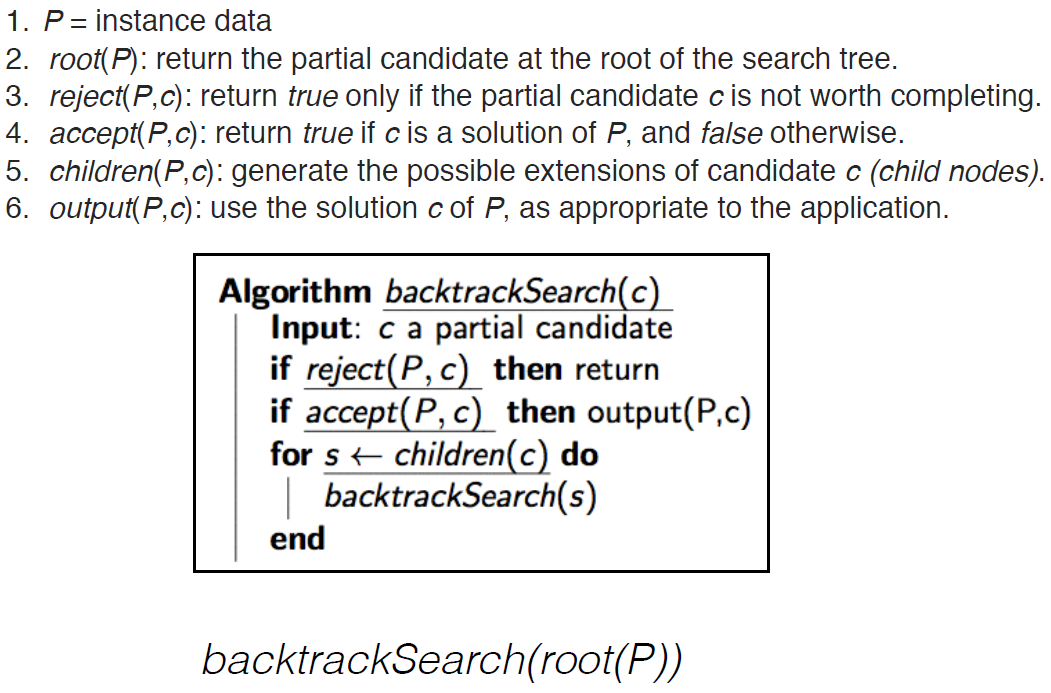
\includegraphics[width=0.8\linewidth]{PseudoCodeBB.png}
    \label{fig:Knapsack_example}
\end{figure}
\FloatBarrier

With the preceding algorithm, a partial solution will be represented as a growing vector
of zero and ones representing whether a given item as been selected or not.

\begin{figure}[!ht]
    \centering
    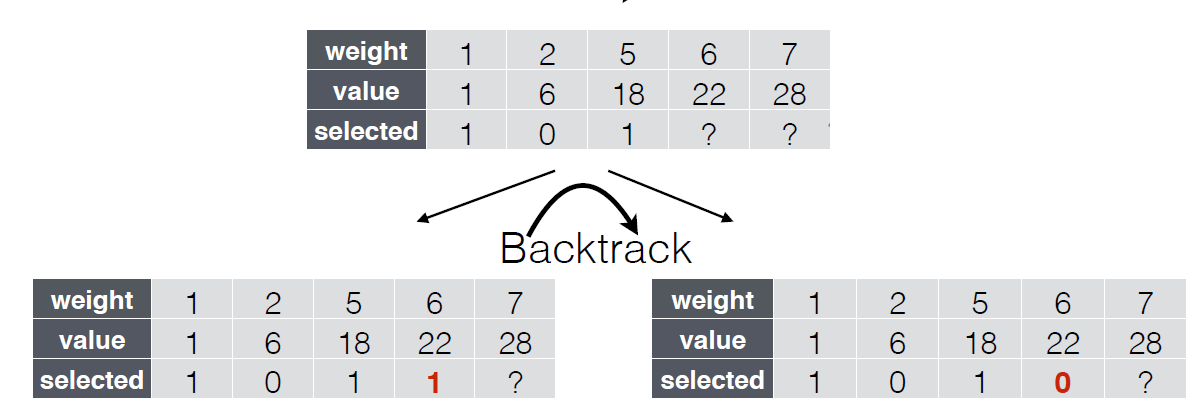
\includegraphics[width=\linewidth]{PartialSolBB.png}
    \label{fig:Knapsack_example}
\end{figure}
\FloatBarrier

This algorithm however has limitations, we must always evaluate the variables of the 
problem in the same order (We cannot affect $X_1$ then$ X_2$ at the left side of the tree 
while on the other side we affect $X_2$ then $X_1$, each level of the tree must strictly 
correspond to the affectation of a variable). As affecting variable in different order may result in better performance, this a limitation.\newline

We also cannot process trees which posses a variable number of children easily with this method. If it was possible we could, for example, decide multiple variable at once
and thus increase the performances of our algorithm. \newline

We must find a way to implement reversible states to improve our algorithm further
by breaking those two limitations. The space usage of those reversible state must however
be relative the the change that have been made on the parent. We do not want to simply
clone the parent and waste memory.

\subsection{Reversible state and magical integers}

\subsubsection{The idea}

To implement those reversible states, we will thus make use of three objects.

\begin{enumerate}
	\item \textbf{ReversibleContext()} : Which will be used to represent a 
	reversible state.
	\item \textbf{ReversibleInt(ReversibleContext rc, int i)} : Which will be used to 
	represent the variables of a reversible state.
	\item \textbf{TrailEntry(ReversibleInt ri, int value)} : Which will be used
	to represent changes on a stacks stocked in the context. This object will
	only be used by the ReversibleContext class.
\end{enumerate}

Using those three object can then implement an reversible context 
which can be used as shown in the following piece of code :

\begin{figure}[!ht]
    \centering
    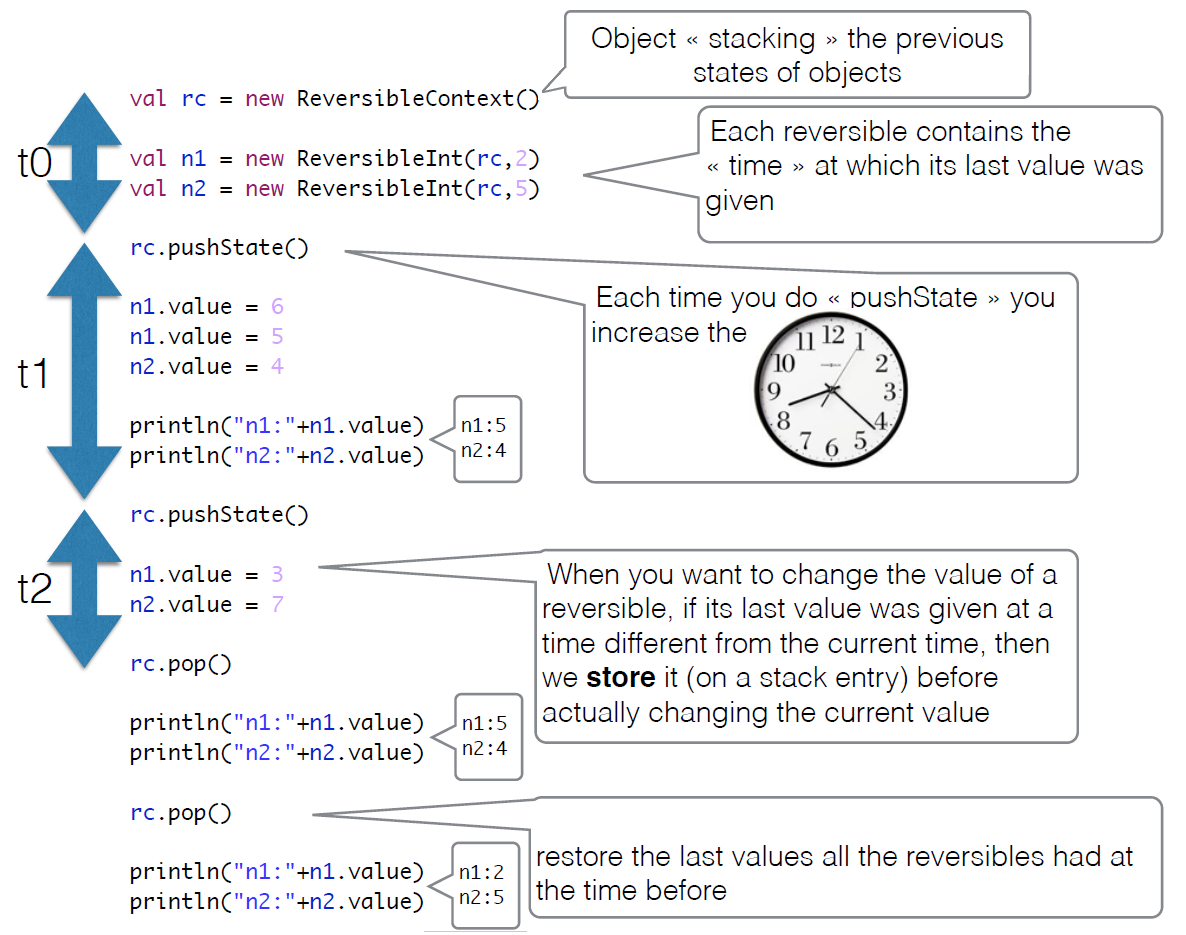
\includegraphics[width=\linewidth]{ReversibleIntegerIntroductionBB.png}
    \label{fig:Knapsack_example}
\end{figure}
\FloatBarrier

With the push pop operation acting as follows:

\begin{figure}[!ht]
    \centering
    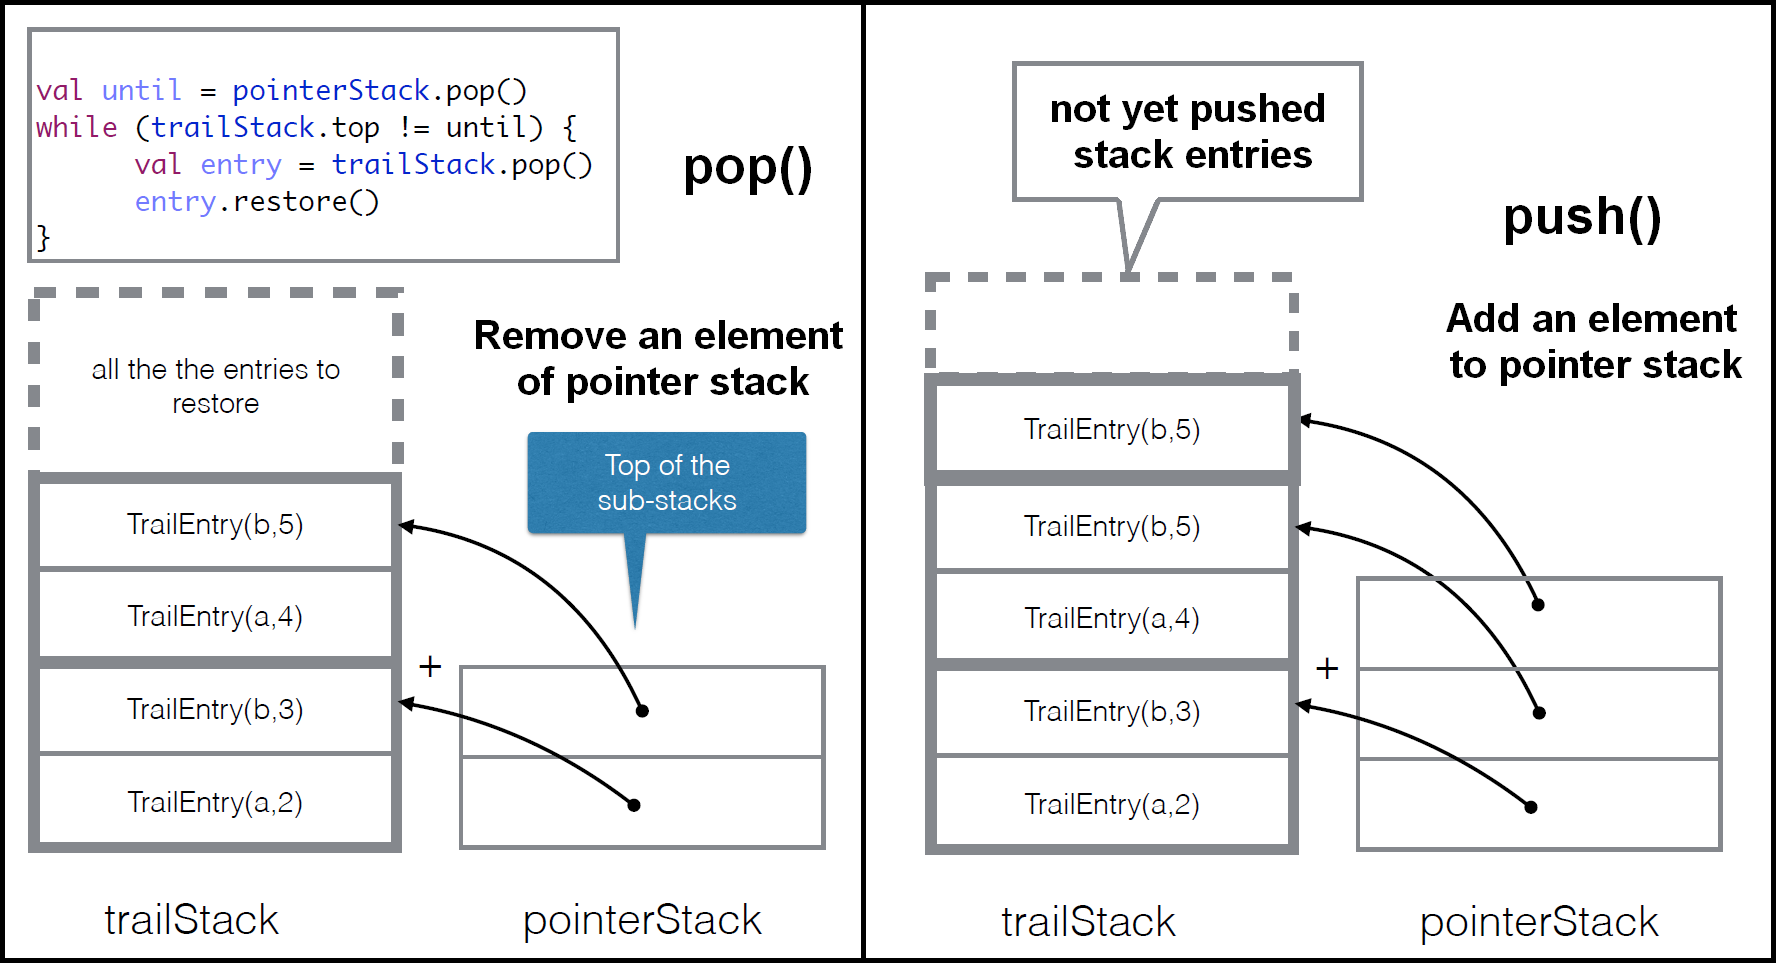
\includegraphics[width=0.9\linewidth]{ReversibleStatePushPop.png}
    \caption{Push/Pop implementation in reversible context}
    \label{fig:Knapsack_example}
\end{figure}
\FloatBarrier

\subsubsection{Implementation}

\#Ca pue l'exam les gars

\begin{figure}[!ht]
    \centering
    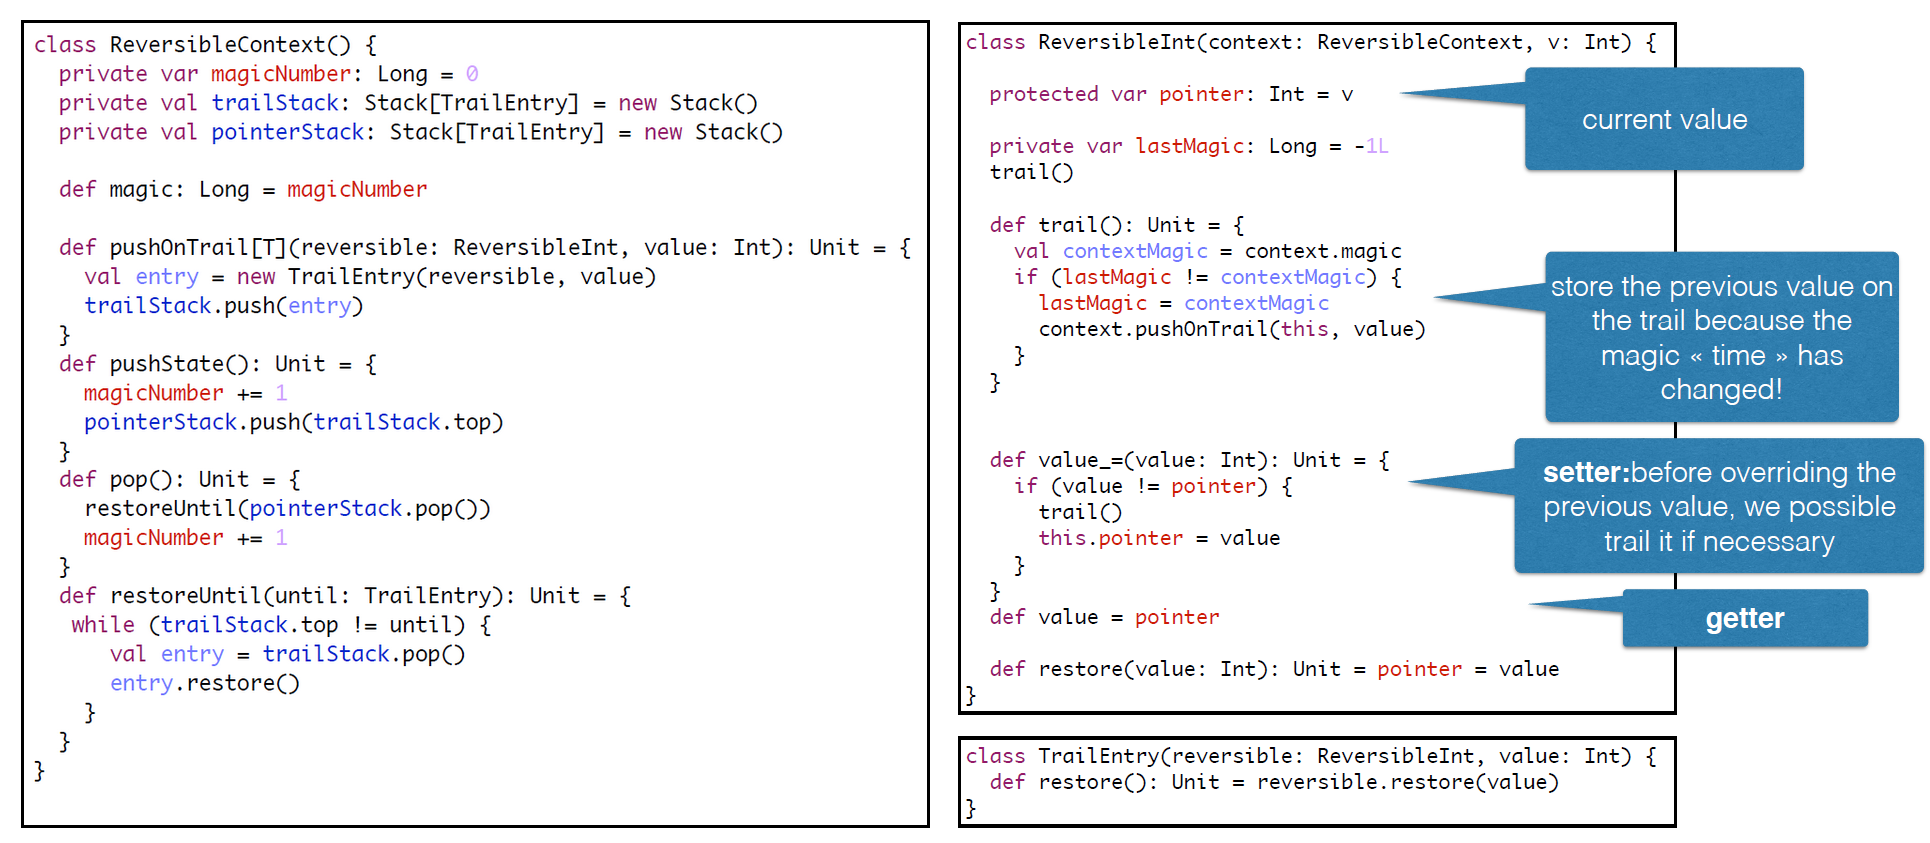
\includegraphics[width=1.1\linewidth]{ReversibleStateImplementation.png}
    \label{fig:Knapsack_example}
\end{figure}
\FloatBarrier

The slides (lecture 2 page 28) contains an implementation of B\&B using branch and bound
which we will not place here as it is highly unlikely that we will be interrogated on it.
Also if you have understood reversible context then it should be fairly easy 
to reimplement in the worst case scenario.

\subsection{Search heuristics}

So far we have always added items on the left side of the tree (affecting variable to 1)
and removed items on the right side. We have also always affected variable sequentially, 
in the same order each time\newline

Now that we can traverse the tree as we want, we can change that and make use of 
heuristics which, at each given moment, decide what variable to instantiate 
and/or which value to assign. 
\newline

In a Branch and bound algorithm, finding good solution faster is better 
as the pruning will become more effective.
Heuristic will also result in a better \textbf{anytime behavior} (the quality of the best
solution you have if you stop the search after a time limit).  \newline

\subsubsection{Iterative Discrepancy Search}

Discrepancy = Number of right (the side in a tree) decisions

If i posses a trustworthy heuristic where interesting sub tree are on the left of a parent,
using a limited discrepancy search would be a good optimisation as wrong decision often
take place in early stages.

\begin{figure}[!ht]
    \centering
    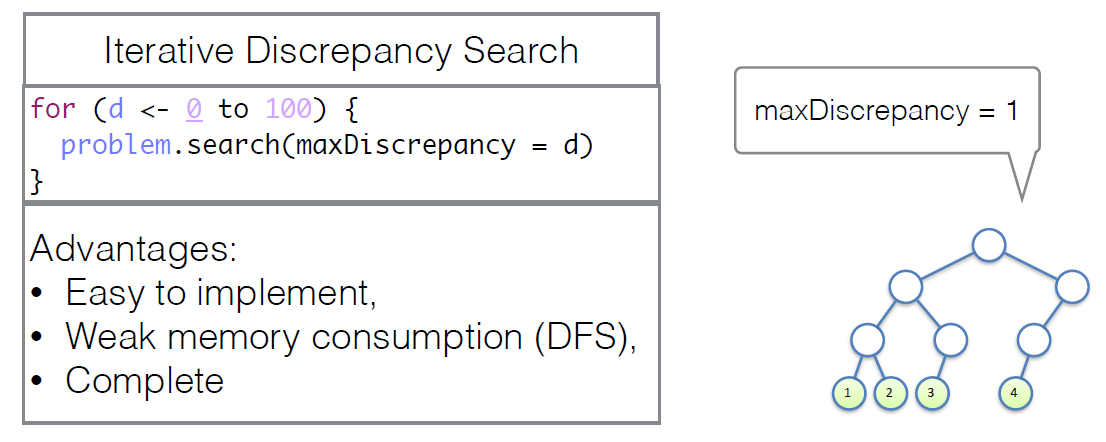
\includegraphics[width=0.8\linewidth]{LimitedDiscrepancySearch.png}
    \label{fig:Knapsack_example}
\end{figure}
\FloatBarrier

As you can see with this method we rapidly find good solution which will help the pruning
during the following iterations. We thus obtain a potentially fast and complete algorithm
(depending on the heuristic). If the heuristic is not significant however the algorithm will
be far slower as it involves much re computation (which normally won't be too signifiant
thanks to the pruning).\newline

\textbf{If the discrepancy search does not explore the tree completely, 
it is not considered complete !} This can however be used as a form of greedy
algorithm.

\subsubsection{Best first search}

Expand the open node with the best upper-bound first (maximization) !
Although fairly efficient and easy to implement, this heuristic has two drawbacks :

\begin{enumerate}
	\item You won't have a feasible solution directly (implication for the pruning).
	\item Memory usage is difficult to control.
\end{enumerate}

\begin{figure}[!ht]
    \centering
    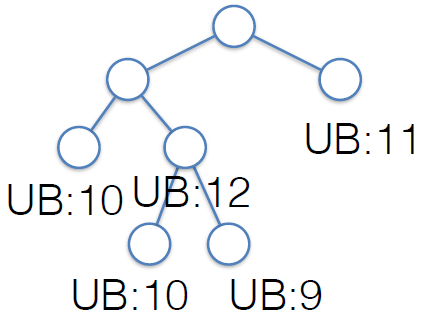
\includegraphics[width=0.3\linewidth]{BestFirstSearchBBHeuristic.png}
    \caption{Representation of the best first search heuristic}
    \label{fig:Knapsack_example}
\end{figure}
\FloatBarrier

\subsubsection{Other heuristics}

TODO

\subsection{Other B\&B optimisations}

\subsubsection{Symmetry detection}

In case of symmetric items in the knapsack set (understand identical), we can reduce the
search space significantly as the items are completely interchangeable.\newline

For example given four symmetrical items $(X_{n+1}, X_{n+2}, X_{n+3}, X_{n+4})$, 
their assignment tree would normally contain 16 elements $(2^4)$ but it can 
be reduced to five due to their symmetrical property. 
We only need to explore the following states:

\begin{enumerate}
	\item (0,0,0,0) => take 0
	\item (1,0,0,0) => take 1
	\item (1,1,0,0) => take 2
	\item (1,1,1,0) => take 3
	\item (1,1,1,1) => take 4
\end{enumerate}

\subsubsection{Dominance detection}

In case an item b is dominated by another item a
(b is dominated by a if $V_a \geq V_b \wedge W_a \leq W_b$)
It is never interesting to take b if a is not also taken ! \newline

An optimal solution cannot have a = 0 and b = 1. 
We can thus avoid to explore such states.

\subsection{Bonus questions and exam questions}

\subsubsection{Reversible set}

\begin{lstlisting}
//WARNING : UNTESTED but the idea is there

//Create ReversibleSet class as follows
// 1 : Add set variable which store curent set
// 2 : Modify pointer to save multiples changes
// 3 : Add remove method which remove in set and adds to changes made
// 4 : Modify trail method to push changes one by one
// 5 : Modifify restore methode to remove unpushed changes and add back argument value
// 6 : Write the get iterator method

class ReversibleSet(context: ReversibleContext, s: Set) {
	protected var currentSet: Set = s //Set
	protected var pointer: Array<Integer> = [] //List of changes
	private var lastMagic: Long = -1L
	trail()
	
	def trail(): Unit = {
		val contextMagic = context.magic
		if (lastMagic != contextMagic) {
			//We need to push values
			lastMagic = contextMagic
			for elem in pointer{ //One push per elem removed
				context.pushOnTrail(this, elem)
			}
			pointer = [] //Reset change array since change have been pushed
		}
	}
	def remove(value: Int): Unit = {
		if (value != pointer) {
			trail() //Always call this method before making changes
			this.currentSet.remove(value) //Remove value in set
			this.pointer.add(value) //Add to changes made
		}
	}
	def getIterator() : Unit = {
		return set.iterator(); //Assuming our set implements iterable
	}
	def set = currentSet //To acces current set value
	
	def restore(value: Int): Unit = {
		//Remove unpushed changes
		for elem in value{
			set.add(elem)
		}
		//(so that we don't add multiple time in case of multiple changes)
		pointer = [] //Reinit change list 
		//Add the value in argument to the set
		set.add(value);
	}
}
\end{lstlisting}

\subsubsection{Explicit stack DFS's pseudo code}

\begin{lstlisting}
//Init stack
stack state_to_visit = new stack();
state_to_visit.add((0,initState)); 
//A tuple (current index, state where no item are taken)
//Init method variable
int maxIndex = nbVariableToAsssign - 1;
state bestSol = initState;
while(!state_to_visit.isEmpty()) {
  (index, state) = state_to_visit.pop();
  if(index > maxIndex){
  	//Computation finished, evaluate state
  	if(bestSol.value < state.value) bestSol = state;
  }
  else if(state.getUpperBound() > bestSol.value){
  	newState = state.makeCopy()
  	//Add current elem not selected state to stack
  	state_to_visit.push((index+1, state));
  	//Add current elem selected state to stack => will be visited first
  	newState.changeElemAtIndex(index, 1); //Set as taken
  	if(newState.isUnderCapacityConstraint()) state_to_visit.push((index+1, newState));
  }
}
return bestSol; 
\end{lstlisting}




\section{Search}
%TODO slides 2


\section{Linear programming}
%TODO slides 3


\section{Lagrangian relaxation}
%TODO slides 4


\section{Network flow}
%TODO slides 5



\section{Greedy and approximation algorithms}


\subsection{An activity-selection problem}
\begin{tabular}{m{6cm}m{10cm}}
    Find the max number of activities that do not
    overlap in time : 
    $$\forall i,j \quad selected: \quad s_i \geq f_j  \quad or \quad s_j \geq f_i$$
    &
\begin{itemize}
    \item $s_i$ = start time of activity
    \item $f_i$ = end time activity (not that activities are 
        sorted such that $f_i \leq f_{i+1}$)
\end{itemize}
\end{tabular}

\begin{enumerate}
    \item \textbf{Reduction} to the maximum independent set problem where 
        we find the maximum set of vertices in a graph such that
        to vertices selected are not adjacent.

        \begin{tabular}{m{10cm}m{3cm}}
            \begin{itemize}
                \item The reduction is done by add an edge between $i$ and $j$ if
                    activities overlap in time: 
                    $$s_i < f_j and s_j < f_i$$ 
            \end{itemize}
            Note that the maximum independent set problem is NP-Hard problem
            &
            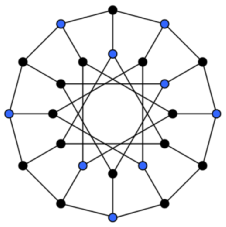
\includegraphics[width=3cm]{img/independant}
        \end{tabular}


    \item \textbf{Dynamic programming}: select a maximum size subset of mutually
        compatible activities from $S_{ij}$, for $0 \leq i < j \leq n+1$,
        knowing that all other $S_{ij}$ are empty.

        $a_m$ such that $f_m = min\{f_k: a_k \in S_{ij}\}$
        \[
            c[i, j] = 
            \begin{cases} 
                0 & \text{if } S_{ij} = \emptyset \\
                max_{\substack{i<k<j \\ a_k \in S_{ij}}} \{c[i, k] + c[k, j] + 1\}  & \text{if } S_{ij} \neq \emptyset
            \end{cases}
        \]
        \begin{itemize}
                %TODO
            \item Time complexity: 
            \item Space complexity: 
        \end{itemize}

        \paragraph{Improvement to a greedy}
        \begin{itemize}
            \item Obs.1: a m is used in some maximum-size subset of
                mutually compatible activities of $S_ij$

                Proof (Sketch):
                \begin{small}
                    Suppose $A_{ij}$ an optimal set of $S_{ij}$ . Take
                    the first activity of $A_{ij}$ (assume it is $a_k$ with $k \neq m$). We
                    can safely replace $a_k$ with $a_m$ because $f_m \leq f_k$.
                \end{small}

            \item Obs.2: The subproblem $S_im$ is empty, so that choosing
                $a_m$ (in the recurrence) leaves the subproblem $S_mj$ as the
                only one that may be nonempty.
        \end{itemize}

        %TODO new recurrence equation

    \item \textbf{Greedy algorithm}
        \begin{lstlisting}[mathescape]
n $=$ nbrActivities
A $= a_1$
i $= 1$

for m $\leftarrow$ 2 to n do
if $s_m \geq f_i$ then
A = $A \cup a_m$
i =$m$

return A
        \end{lstlisting}
\end{enumerate}


\subsection{Greedy}
At each decision point, the algorithm makes
a \textbf{local optimum choice} in the hope that it is a global
optimum choice.
\begin{itemize}
    \item For some problem it's the case
    \item For other it's not and sometimes we can 
        have a guarantee how
        \textit{suboptimal} we can be.
\end{itemize}


\subsection{Minimum Spanning Tree (MST)}

\subsubsection{Definition}
\begin{itemize}
    \item A \textbf{cut} (S,V-S) of an undirected graph
    \item An edge (u,v) \textbf{cross} the cut (S,V-S) if one of its
        endpoints is in S and the other in V-S
    \item A cut \textbf{respects} a set A of edges if no edge in A crosses
        the cut.
    \item An edge is a \textbf{light edge} crossing a cut if its weight is
        the minimum of any edge crossing the cut. (can be
        more than one in case of ties).
\end{itemize}

\subsubsection{Theorem}
\begin{itemize}
    \item[LET]
    \item $G=(V,E)$ a undirected graph with weight function $w$ on $E$.
    \item $A \subseteq E$ included in some MST for $G$.
    \item $(S, V-S)$ be any cut of $G$ that respect $A$
    \item $(u,v)$ be a light edge crossing $(S, V-S)$
    \item[THEN]
    \item edge $(u, v)$ is safe for $A$
\end{itemize}

\paragraph{Proof}
Let $T$ be a minimum spanning tree that includes $A$, and assume
that $T$ does not contain the light edge $(u,v)$, since if it does we
are done.

\begin{enumerate}
    \item Because $(u,v)$ are on opposite sides
        of the cut $(S,V-T)$ that respects $A$,
        there is necessarily some edge $(x,y)$
        on path $p$ also on opposite sides of
        the cut.

    \item We can form an other MST $T'$ by
        removing $(x,y)$ and adding $(u,v)$ from
        $T$. Because when considering $A$,
        $(u,v)$ is a light edge, $(x,y)$ cannot be
        cheaper than $(u,v)$ (by definition of a
        light edge).
\end{enumerate}


\subsubsection{Algorithm}

\begin{lstlisting}[mathescape, caption=Generic-MST(V\,E\,c\,s\,t)]
A = $\emptyset$
while A does not form a spanning tree do
    find an edge $(u, v)$ that is safe for A
    A = A $\cup \{(u, v)\}$

return A
\end{lstlisting}

\begin{itemize}
    \item \textbf{Kruskal}  
        
        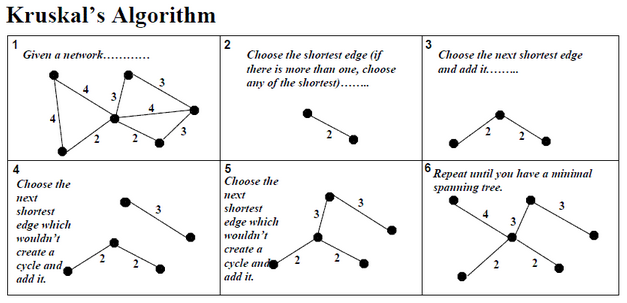
\includegraphics[width=14cm]{img/kruskalAlgo}
    \item \textbf{Prim} 
        
        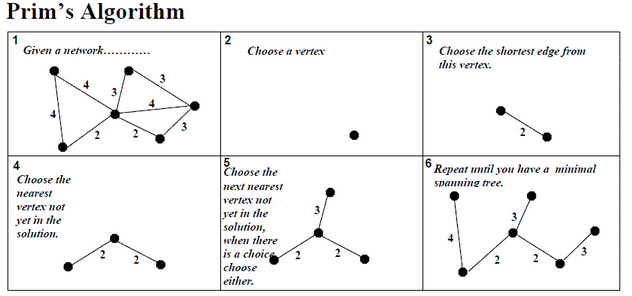
\includegraphics[width=14cm]{img/primAlgo}
\end{itemize}

\subsubsection{Implementation using disjoint-set forests}
Kruskal and prim can be implemented in $O(E \times log(V))$

\begin{lstlisting}[mathescape, caption=MST-Kruskal(G\,w)]
A = $\emptyset$
for each vertex $v \in V$ do
    Make-Set-(v)

sort the edge of $E$ into non decreasing order by weight $w$
for each edge $(u,v) \in E$ taken in non decreasing order by weight do
    if Find-Set(u) $\neq$ Find-Set(v) then
        A = A $\cup \{(u, v)\}$
        Union(u,v)

return A
\end{lstlisting}

\begin{center}
\begin{tabular}{m{7cm}m{7cm}}
    \begin{lstlisting}[mathescape]
MAKE-SET(x)
    X.p = x
    x.rank = 0

FIND-SET(x)
    if x $\neq$ x.p
        x.p = fIND-SET(x.p)
    return x.p
    \end{lstlisting}
    &
    \begin{lstlisting}[mathescape]
UNION(x, y)
    LINK(FIND-SET(x), FIND-SET(y))

LINK(x, y)
    if x.rank > y.rank
        y.p = x
    else 
        x.p = y
        if x.rank == y.rank
            y.rank = y.rank + 1
    \end{lstlisting}\\
    $\rightarrow$ Path compression
    & 
    $\rightarrow$ Union by rank
\end{tabular}
\end{center}

\begin{itemize}
    \item \texttt{Sort} in $O(E \times log(E)) = O(E \times log(V^2)) = O(E \times log(V))$
    \item \texttt{Make-Set(x)}: make a set with $x$
    \item \texttt{Find-Set(x)}: return pointer to the set containing $x$

        \paragraph{O(1)} is assured by using \textbf{path compression}.

        \begin{tabular}{m{11cm}m{3cm}}
            During Find-Set operation, make each node
            on the find path point directly to the root
            &
            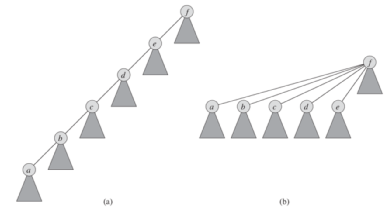
\includegraphics[width=3cm]{img/compression}
    \end{tabular}


    \item \texttt{Union(x, y)}: merge two sets (can't have a duplicate element
        because of set)

        \paragraph{O(1)} is assured by using \textbf{union by rank}.

        \begin{tabular}{m{11cm}m{3cm}}
            Make the root of the tree with the fewer nodes points to
            the root of the tree with more nodes.
            &
            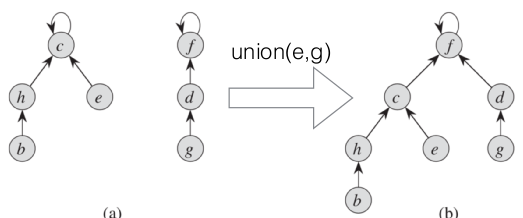
\includegraphics[width=4cm]{img/union}
    \end{tabular}
\end{itemize}

\begin{itemize}
    \item The time complexity of $m$ (> n) operations on $n$ objects
        using Disjoint-set forests implemented with path
        compression and union by rank $i$: 
        $$\Theta(m \alpha(m,n))$$
    \item $\rightarrow \alpha(m, n)$ is the inverse Ackermann's function. 
        In fact, it's less than 5 for any practical input size $n$
\end{itemize}

\subsection{Approximation}

An algorithm for a problem has an \textbf{approximation ratio} of $\rho(n)$ if
for any input size $n$, the cost $C$ of the solution is within a factor
$\rho(n)$ of the cost C* of an optimal solution.
$$max(\frac{C}{C*}, \frac{C*}{C}) \leq \rho(n)$$

\subsubsection{Set cover example}
Minimum set of vertices such that each
edge of the graph is incident to at least one vertex of
the set.

\begin{lstlisting}[mathescape, caption=Greddy set cover]
C = $\emptyset$
E' = G.E
while E' $\neq \emptyset$ do
    $(u, v)$ be arbitrary edge of E'
    C = C $\cup \{u, v\}$
    remove from E' every edge incident on either $u$ or $v$

return C
\end{lstlisting}

%TODO slide 29 et + lecture 06
TODO slide 29 et + lecture 06

\subsubsection{Subset-sum}

\subsection{Exam}
\begin{itemize}
    \item All theoretical notions introduced (proofs, etc).
    \item Design a greedy algorithm
    \item MST: I give you a new MST greedy algorithm. You
        should be able argument whether it is correct or not.
    \item Design a simple approximation scheme, compute it’s
        approximation ratio
    \item I give you a complexity of an approximation scheme.
        You should be able to tel me if it is fully polynomial.
\end{itemize}



\section{Local search}
%TODO slides 7


\section{Constraint programming}
%TODO slides 8


\section{Local Neighbors Search}
%TODO slides 9


\section{Derivative free optimization}
%TODO slides 10


\section{Bi-objective}
%TODO slides 11




\end{document}
